\chapter{Boss development}
\section{Introduction}
BOSS had been used since 2002 within CMS production~\cite{citeulike:877254} and in DC04 with analysis~\cite{CHEP04_TALLINI, citeulike:876380}. After DC04 it was decided that BOSS would be integrated into both systems to provie generic batch job functionality. The opportunity was taken to re-design BOSS completely to fit this role better, existing functionality was improved and new features introduced~\cite{citeulike:880984}. New features included the concept of a task and the possibility for a job to run more than one application. Improvements were made to the monitoring (removing the direct database connection) and logging (eliminating the requirement for a database server). 

%%%%%
%ituent jobs and allowing a job to run more than one user application (so called job-chainning) in a user defined workflow. Many other improvements and refinements were introduced; improved logging (removing the need for a MySQL database server), improved monitoring (removing the direct database connections from jobs).
%%%%%
\section{Limitations of previous versions}
%. These experiences pinpointed various limitations and possible improvements. Some of the proposed changes implied large scale architectural changes i.e. support for the task concept.

The lack of a task hierarchy required both CMS production and analysis systems to operate BOSS with an ensemble of individual jobs. A separate BOSS invocation was required for each job, with no sharing of information between instances.

The BOSS API did not offer any greater functionality or control than the command line client. The only available operations were the high level command's accepted by the command line, i.e. job creation and submission. To get feedback from the operation the calling application had to parse the commands output. The API was implemented only in C++ and thus was unavailable to the large amounts of CMS software written in other languages. As a consequence both CRAB and the Monte Carlo production system ignored the API and used the command line client.
% It was thus decided to replace this API with one that had much greater functionality and finer grained control. This API would also be implemented in multiple languages widening its availability.

%  required the calling program to place the same options as would have been passed on the command line into a string and simply pass these to the API. The API provided no extra functionality or control than the command line. Only a C++ API existed thus it was only convenient for other C++ programs to call. Thus there was very little benefit to using the API. It was decided to replace this with an API which had much more functionality and could be implemented in many languages.

Installation was complicated by the requirement for a MySQL database. This provided a central logging repository but a database server was seen as unnecessary for the average user. It was not possible to automate the installation so this step had to be performed by the user. In principle it was possible for everyone in CMS to share the same database server however firewalls, concerns over a single point of failure and load issues ruled this out in practice. Thus generally either a user or site setup their own database which was used by that user or all users at the site.

%It was proposed to modify this requirement to any database implementation that understood SQL. This provided the opportunity to use embedded databases. Embedded databases used the local filesystem for data storage but had no server component: access was only available via an application or API on the local machine. 

% The idea was proposed to allow different database backend technologies, thus the default would be a lightweight file based database but users who needed greater performance could choose a heavy weight database implementation.

The reliability and robustness of the logging and monitoring information were reduced by reliance on a direct connection from the running job back to the MySQL database. This could be blocked by either site with a firewall. If the connection could not be established then neither monitoring nor logging information would be saved. Once the job had finished and the user had access to the output they could run a BOSS command over the journal file and populate the database. This operation required manual intervention, which could not be guaranteed and only provided monitoring information at the end of the job. 
%The logging and bookeeping mechanisms were improved with the primary goal of guaranteeing the reliability of the logging information.



%This had the disadvantages that a user had to know that information was missing and manually run a command. Also not all information was always populated correctly. 

%%%%%
%o seperate jobs no idea of hierarchy
%o crappy api
%o crappy monitoring
%o crappy logging - if no db connection
%o crappy install - MySQL
%%%%%
\section{New Architecture}
Both the CMS analysis and production workflows involved a single computational task split into multiple jobs, each of which was largely identical. Previous BOSS versions were unaware of any relationship or commonalities between jobs, which required the calling application to invoke BOSS separately for each job. Hence it was decided by the author to introduce support for groups of jobs with the task concept. This would allow the calling application, or user, to operate at a higher level of abstraction.
 
%Most BOSS operations by the anlysis and production frameworks involved multiple jobs thus a higher level abstraction allowed for a simpler interface between the two. Hence it was decided to introduce support for groups of jobs, tasks.

Previously jobs were limited to running a single executable. Clients who required more functionality were forced to submit a script that executed their workflow. This forced the entire workflow to be recorded as a single execution with no monitoring of individual components. It was therefore decided to modify BOSS to run an arbitrary number of fully configurable applications in a single job. 

The new default behaviour was to run the job's applications in a linear chain, although more complicated workflows were also supported. It was envisaged that this workflow could be dynamically steered by the conditions on the worker node and the success or failure of the applications. This had many advantages for jobs where pre-programmed actions could be taken if certain error conditions were met. This kind of self-aware job would be increasingly useful as the number of jobs submitted by CMS increased to maintain a manageable number of failures. 

The chaining process was complex, with differing user requirements. On account of this complexity it was decided to provide a plug-in mechanism for the chainer. A basic chainer was provided that ran the user's applications in a linear chain. If users required greater functionality they could provide their own. The chainer configuration was inserted into the BOSS task description and passed transparently down to the chainer at run time. 

Previously job resubmissions overwrote all information concerning previous executions, resulting in an incomplete activity record. To correct this the logical job concept was separated from physical executions. Within a task jobs could be executed multiple times with the database reflecting this. In the logical view the ``job'' was renamed ``chain'' to reflect the idea that more than one application (``program'') could run in the workflow. The execution view consisted of ``jobs'' each composed of multiple ``program executions''. For each submission of a ``chain'' the database contained a different ``job''. The user could query the ``chain'' and be provided with a complete history of the submitted ``jobs''.

Previously there had been no difference between logging and real time monitoring information. Both were stored in the database via a direct connection from the running job. This was unreliable, unscalable and ignored the differences between logging and real time monitoring. Hence it was decided to separate these different types of information. Logging information availability and integrity were guaranteed while monitoring was optional and collected if possible.

As the logging database was no longer required to accept connections from running jobs the need for a database server was eliminated. The central MySQL server was replaced by a plug-in mechanism that allowed any SQL-compatible database to be used. This provided the opportunity to use embedded databases. Embedded databases used the local filesystem for data storage but had no server component: access was only available via an application or API on the local machine. The new default was to use an embedded database this simplified the installation process and eliminated a potential security vulnerability. Due to the plug-in mechanism users could still, if they wished, use a database server. 

Logging information could only be added to the logging database by the BOSS client tools. Logging information from a job was obtained from the journal file and was retrieved at the end of the job. The same BOSS command that retrieved output from a job parsed the journal file and updated the logging database. This was automatic and required no manual intervention by the user.

\begin{figure}[tbp]
  \centering
  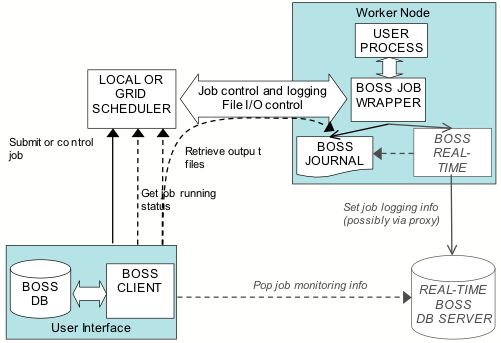
\includegraphics[width=0.85\linewidth]{boss/boss_information_flow}
  \caption{New BOSS information flow.~\cite{citeulike:880984}
  \label{fig:boss_information_flow}}
\end{figure}

Monitoring was optional and the information returned via a monitoring database server. These databases could be installed by the individual user or, more likely, by a Tier-1/2 for all its users. Information was sent from jobs to the dedicated monitoring server via a specialist monitoring framework. Multiple frameworks were available including a custom protocol~\cite{citeulike:880984} and MonaLisa~\cite{citeulike:880975}. Information would then reside in this database until retrieved by the user with the BOSS client. The monitoring information had a limited lifetime and could not be used to populate the logging database.

Figure~\ref{fig:boss_information_flow} shows the new BOSS components and information flow. The constituent jobs in the task were submitted via a batch scheduler to a worker node. Once the job started BOSS activated the monitoring and chainer. The chainer took responsibility for the users workflow, as illustrated in Figure~\ref{fig:boss_chain}. Logging and monitoring information were written to the journal file and, if requested by the user, sent to the monitoring database. The user BOSS client tools retrieved information from the monitoring database and hence allowed users to track their jobs. Once the job finished the user retrieved the output and BOSS updated the logging database from the journal file.

%show picture - BOSS architecture pic
\begin{figure}[!tp]
  \centering
  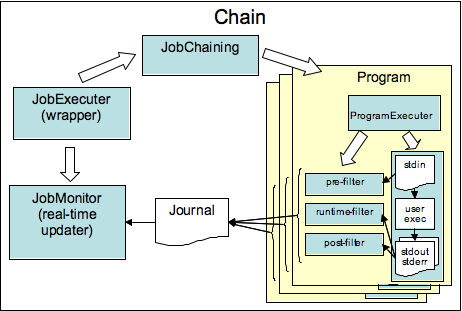
\includegraphics[width=0.85\linewidth]{boss/boss_chain}
  \caption{BOSS runtime components.~\cite{citeulike:880984}
  \label{fig:boss_chain}}
\end{figure}

\section{Task Definitions}
To create a task the user required a syntax that could express the hierarchy. A logical choice for this was XML, which naturally provides for nested hierarchies of tasks, jobs and applications. Figure~\ref{fig:boss_xml} shows an example task specification. This shows a task composed of 100 chains each composed of one program. The ``iterator'' concept was introduced to simplify writing specifications. This provided a looping mechanism within the specification. The iterator was replaced by the required number of chains (or other inner element) and the iterator name was replaced by its value as of that loop iteration. 

%\begin{figure}[!tp]
%  \centering
%  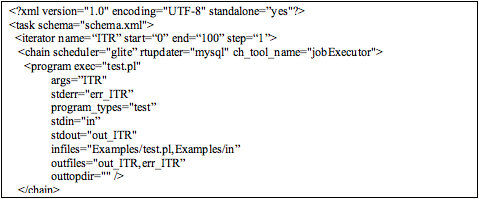
\includegraphics[width=0.85\linewidth]{boss/boss_xml}
%  \caption{An example XML task specification showing a task composed of 100 chains of one program.~\cite{citeulike:880984}
%  \label{fig:boss_xml}}
%\end{figure}
\begin{figure}[!tp]
\begin{verbatim}
<?xml version="1.0" encoding="UTF-8" standalone="yes"?>
	<task schema="schema.xml">
	  <iterator name="ITR" start="0" end="100" step="1">
	   <chain scheduler="glite" rtupdater="mysql" ch_tool_name="jobExecutor">
	     <program exec="test.pl" 
	              args="ITR" 
	              stderr="err_ITR"
	              program_types="test"
	              stdin="in"
	              stdout="out_ITR"  
	              infiles="Examples/test.pl,Examples/in"
	              outfiles="out_ITR,err_ITR"
	              outtopdir="" /> 
	   </chain>
	  </iterator>
	</task>
\end{verbatim}
\caption{An example XML task specification showing a task composed of 100 chains of one program.~\cite{citeulike:880984}\label{fig:boss_xml}}
\end{figure}
There were two standard XML parsing mechanisms: Document Object Model (DOM) and Simple Api for Xml (SAX). DOM provided a navigable object tree representing the document. SAX provided an event-driven system for calling a given function when a certain tag was encountered. For instance when a task definition was encountered, a function would be called to instantiate a task object. There were advantages and disadvantages to both methods: SAX was generally faster but required development of functions to create tasks and jobs (which would need updating with any schema changes) whereas DOM provided the entire document as an accessible object but had greater memory requirements. 

It was decided that the greater speed of SAX was unnecessary for this project as users would generally only create tasks with O(1000) jobs and communication with external services, PubDB and LCG, would dominate any latencies. Due to the predicted size of users tasks the possible higher memory use of DOM was not considered a problem. Thus it was decided to use DOM with the document object as the internal task data structure. This was an idea taken from web browsers where internally an HTML page is stored as a DOM object. In the future when more users create larger tasks these performance issues may become important however it was viewed that in the short-medium term these performance issues were not be important.

%Once the choice of parsing method had been made the choice of parser implementation remained. Several mature parser libraries which could handle both DOM and SAX existed. Requirements included ease of install and wide availability amongst LCG sites (It was required at runtime to allow the chain to read its workflow). In order to allow the DOM object to be used for the task representation it was desirable for BOSS to be able to obtain pointers directly at a tasks children i.e. the chains and their children i.e. the executables. This would allow the passing of a start and end pointer to functions that operated on a subset of the chains. This violated the object orientedness of the system and only a few libraries could be used in this way.

%CMS and LCG had decided on Xerces produced by the Apache foundation. This was a mature and very capable library however it involved a reasonable install (11MB), was fairly complicated and did not provide the facility that would allow BOSS to get direct access to a documents children. For these reasons another parser was chosen, libxml2. This has been developed by the Gnome project and is a C library that provided mechanisms for directly accessing the children of a documnet.

%Wrapping the XML libraries was a BOSS class called XMLDoc. This class provided all neccesary functions for BOSS including parsing, attribute/child modification and the ability to obtain pointers (of the same type) to children that statsfied a query.

The iterator concept required either support from the task object or modification of the XML before parsing because XML does not support the concept of iterators. The latter could be achieved by use of Extensible Stylesheet Language Transformations (XSLT). This is a language capable of describing transformations of an XML document and is usually used to convert XML to viewable HTML. XSL transforms were designed to execute certain actions when a particular XML structure was encountered, but XSL lacks support for loop structures and did not fully support variable modification. The combination of these resulted in a limit of one iterator tag. If more than one tag was included in a document the two would interfere and only the values of one would be correctly replaced. This was not regarded as a major limitation because the most common usage was a single iterator of chains within a task.

%The GNOME project also provided an XSLT library called libxslt.

%XSL transforms were designed for parsing XML and outputting certain strings when a particular piece of XML is reached not for implementing loop structures. A way round this was found but resulted in the limitation of a maximum of one iterator tag, this was because it couldn't correctly replace the text in both iterations only the last iterators text was replaced. This wasnt a problem as most use involved a single iterator cycling over the chains in a task.

\section{API}
The previous BOSS API provided the same commands as the command line client with no fine-grained control or feedback. It was decided that a more complete API that allowed greater control and functionality was required.

% BOSS was written in C++ so a C++ API could be used by the BOSS CLI and external clients.

The API needed to provide functionality suitable for CMS analysis, production and individual users. The API was split into two: user commands (e.g. submit, query) and administration tasks (e.g. register scheduler, job types). The administrator commands could only be run by someone with database administrator privileges. 

%The Administrator commands included registration of job types, batch schedulers and chainer tools. 

%The user API provided the facility for task declaration, submission, querying and output retrieval.

As with the rest of BOSS these API's were written in C++. However, both the CMS production and analysis frameworks were written in Python. It is possible for a Python program to call a C++ API but this required significant effort on the part of the client developer. As a number of CMS applications, both current and proposed, were written in Python it was decided to provide a Python version of the API's. It was felt that the best way to do this was to wrap the C++ API hence ensuring that the two were continually synchronised. 

The wrapping code had to provide a number of features, including:
\begin{itemize}
\item Input argument validation;
\item Conversion of input Python arguments to C++ datatypes;
\item Invocation of the corresponding C++ method; and
\item Conversion of output values to Python datatypes.
\end{itemize}

Advanced C++ features such as polymorphism and exception handling required more complex wrapping code. This problem had been encountered before in computer science and a number of tools had been developed to automate the process. These included SWIG~\cite{citeulike:881608}, SIP~\cite{citeulike:881611} and BOOST.Python~\cite{citeulike:881616}. These tools could generate Python code from the C++ sources and their use was less error prone and faster than writing the code manually.

Each tool implemented a slightly different wrapping strategy. SWIG generated wrapper code from the C++ header files that was then built against the C++ libraries. It had support for multiple scripting languages including Python, Perl, Ruby and many others, and was widely adopted with good documentation. 

SIP was originally designed to generate Python bindings for a graphical user interface. It used a similar method to SWIG with separate wrapper code generation and build steps. It had the disadvantages that it was specifically designed for one application and not as a general-purpose tool. It also only worked with Python and had minimal documentation. 

BOOST.Python took a different approach, called template metaprogramming, where each function was declared in Python with a special syntax. By calling this function BOOST automatically called the appropriate C++ code. This required a modern compiler to work correctly and only supported the Python language.

%The wrapping added a significant overhead to any function call however this was likely to be small compared to the overheads associated with communication with the database and batch scheduler. ref study on speed.

Due to the documentation and the support for multiple languages it was decided to use SWIG to create the API bindings. The wrapping added a significant overhead to any function call and SWIG was considerably slower than the other tools~\cite{citeulike:881635}. However this overhead was expected to be small compared to the overheads associated with database or scheduler communication as a typical session involved O(10) Python method calls.

%however this was likely to be small compared to the overheads associated with communication with the database and batch scheduler. SWIG was considerably slower than other methods however as a typical session involved O(10) Python method calls the effect was acceptable~\cite{citeulike:881635}.

%%%%%
% Do we need the details?
%SWIG required directing by a file listing the Python module to build and the functions to wrap. This was simplified as you could simply tell SWIG to include the contenets of the C++ header file.
%%%%%

Only the generation of the Python bindings required SWIG, while the building and linking did not. The generation step was performed by a developer during the building of a release. With the generated code added to the release the user only needed to build everything together. Thus there was no requirement for SWIG to be available on the user's machine. 
%Binary distribution was also available.


% emphasize diff between distributing source code and binaries

%%%%%
%Problems with previous versions
%Problems encountered by GROSS
%improvements from GROSS
%Others - i.e. chainning
%
%New Architecture
%
%XML task specification
%DOM
%Original idea to have XML DOM represent task i.e. like web page - ref and show feasible
%libxml2 - easy and common
%requirement for ability to go down hiearchy modifying (what about rest - why?)
%transform - iterator - not ideal - limitation
%
%Pyhton API for CRAB + ProdAgent
%%%%%

\section{Conclusion}
Use by both the CMS production and analysis systems required a number of enhancements to BOSS. These included the task concept and better logging mechanisms. An improved API was introduced with greater functionality and multi-language support. To support the task structure a new XML-based task specification was developed. 
